\documentclass[11pt,letterpaper,boxed]{pset}

\usepackage[margin=0.75in]{geometry}
\usepackage{ulem}

\begin{document}

    \problemlist{PHYS051 HW07}
    \begin{center}
        P33.12, P33.13
    \end{center}
    
    \begin{problem} [P33.12]
    A conductor consists of an infinite number of adjacent wires, each infinitely long and carrying a current $i$. Show that the lines of $\Vec{B}$ are as represented in Fig. 33-61 and that $B$ for all points above and below the infinite current sheet is given by \[B = \frac{1}{2}\mu_0ni\]
    where $n$ is the number of wires per unit length. Derive both by direct application of Ampere's Law and by considering the problem as a limiting case of Sample Problem 33-5.
    \end{problem}
    
    \begin{figure*} [ht]
        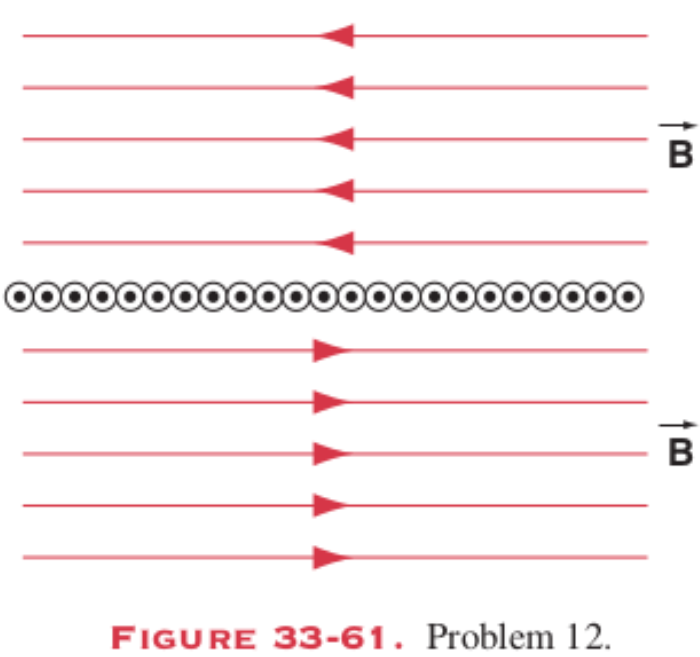
\includegraphics[width=125px]{HW7Images/P33-12.png}
        \label{fig:P33-11}
    \end{figure*}
    \newpage
    
    \begin{problem} [Sample Problem 33-5]
    Figure 33-14 shows a flat strip of copper width $a$ and negligible thickness carrying a current $i$. Find the magnetic field $\Vec{B}$ at point $P$, at a distance $R$ from the center of the strip along its perpendicular bisector.
    \end{problem}
    
    \begin{figure*} [ht]
    \centering
        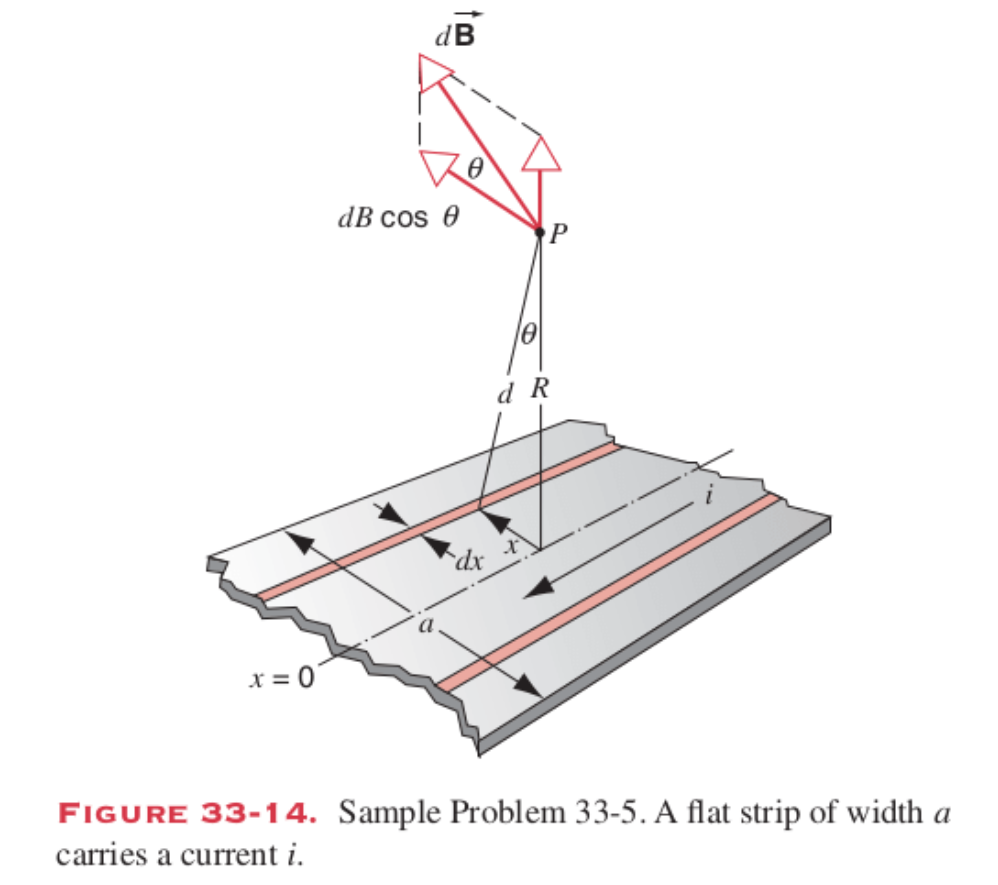
\includegraphics[width=125px]{HW7Images/33-5.png}
        \label{fig:P33-5}
    \end{figure*}
    
    \begin{solution}
    Let us subdivide the strip into long, infinitesimal filaments of width $dx$, each of which may be treated as a wire carrying a current element $di$ given by $i(dx/a)$. For the current element in the left half of the strip in Fig 33-14, the magnitude $dB$ of the field at $P$ is given by the differential form of Eq. 33-13, or 
    \[db = \frac{\mu_0di}{2\pi d} = \frac{\mu_0i(dx/a)}{2\pi R \text{sec}\theta}\]
    in which $d=\frac{R}{\text{cos}\theta}=R\text{sec}\theta$. Note that the vector $d\Vec{B}$ is at right angles to the line marked $d$. 
    
    \smallskip
    Only the horizontal component of $d\Vec{B}$ -- namely, $dB \text{cos}\theta$ -- is effective; the vertical component is canceled by the contribution of a symmetrically located current element on the other side of the strip (the second shaded element in Fig. 33014). Thus $B$ at point $P$ is given by the (scalar) integral 
    \[B = \int dB \text{cos} \theta = \int \frac{\mu_0i(dx/a)}{2\pi R \text{sec}\theta}\text{cos}\theta = \frac{\mu_0i}{2\pi aR}\int \frac{dx}{\text{sec}^2\theta}\]
    
    The variables $x$ and $\theta$ are not independent, being related by 
    \[x = R \text{tan} \theta \text{or} dx = R \text{sec}^2\theta d\theta\]
    
    The limits on $\theta$ are $\pm \alpha$, where $\alpha=\text{tan}^{-1}(\frac{a}{2R})$. Substituting for $dx$ in the expression for $B$, we find
    
    \[B = \frac{\mu_0i}{2\pi aR} \int \frac{R \text{sec}^2\theta d\theta}{\text{sec}^2\theta} = \frac{\mu_0i}{2\pi a} \int^{+\alpha}_{-\alpha}d\theta = \frac{\mu_0i}{\pi a}\alpha = \frac{\mu_0i}{\pi a}\text{tan}^{-1}\frac{a}{2R}\]
    
    This is the general result for the magnetic field due to the strip.
    
    \smallskip
    At points far from the strip, $\alpha$ is a small angle, for which $\alpha \approx \text{tan} \alpha = \frac{a}{2R}$. Thus we have, as an approximate result, 
    
    \[B \approx \frac{\mu_0ia}{2\pi aR} = \frac{\mu_0i}{2\pi R}\]
    
    This result is expected because at distant points the strip cannot be distinguished from a thin wire.
    \end{solution}
    \newpage
    
    \begin{problem} [P33.13]
    The current density inside a long, solid, cylindrical wire of radius $a$ is in the direction of the axis and varies linearly with radial distance $r$ from the axis according to $j = j_0\frac{r}{a}$. Find the magnetic field inside the wire. Express your answer in terms of the total current $i$ carried by the wire.
    \end{problem}
    \newpage
\end{document}